%%%%%%%%%%%%%%%%%%%%%%%%%%%%%%%%%%%%%%%%%%%%%%%%%%%%%%%%%%%%%%%%%%%%%
% LaTeX Template: Project Titlepage Modified (v 0.1) by rcx
%
% Original Source: http://www.howtotex.com
% Date: February 2014
% 
% This is a title page template which be used for articles & reports.
% 
% This is the modified version of the original Latex template from
% aforementioned website.
% 
%%%%%%%%%%%%%%%%%%%%%%%%%%%%%%%%%%%%%%%%%%%%%%%%%%%%%%%%%%%%%%%%%%%%%%

\documentclass[11pt]{article}
%\usepackage[a4paper]{geometry}
\usepackage[left=1.5cm,right=1.5cm,top=2cm,bottom=2cm]{geometry}
\setlength\parindent{0pt}
\setlength{\parskip}{1em}
\usepackage[table,xcdraw]{xcolor}
\usepackage{fancyhdr}
\usepackage{helvet}
\usepackage{lastpage}
\usepackage{graphicx, wrapfig, setspace, booktabs}
\usepackage{titlepic}
\usepackage[T1]{fontenc}
\usepackage[font=small, labelfont=bf,center]{caption}
\usepackage{fourier}
\usepackage[protrusion=true, expansion=true]{microtype}
\usepackage[english]{babel}
\usepackage{sectsty}
\usepackage{url, lipsum}
\usepackage{multirow}
\usepackage{float}
\usepackage{amsmath}
\usepackage{bm}
\usepackage{subfig}
\usepackage{tikz}
\usepackage{svg}
\usepackage[final]{pdfpages}
\usepackage{hyperref}
\usepackage[all]{hypcap}
\newcommand{\HRule}[1]{\rule{\linewidth}{#1}}
\onehalfspacing
\setcounter{tocdepth}{5}
\setcounter{secnumdepth}{5}

%-------------------------------------------------------------------------------
% HEADER & FOOTER
%-------------------------------------------------------------------------------
\pagestyle{fancy}
\fancyhf{}
\setlength\headheight{15pt}
\fancyhead[L]{iz16368}
\fancyhead[R]{University of Bristol}
\fancyfoot[R]{Page \thepage\ of \pageref{LastPage}}
%-------------------------------------------------------------------------------
% TITLE PAGE
%-------------------------------------------------------------------------------

\begin{document}

\title{ \normalsize \textsc{Advanced Space Systems}
		\\ [2.0cm]
		\HRule{0.5pt} \\
		\LARGE \textbf{\uppercase{New Horizons GMAT Coursework}}
		\HRule{2pt} \\ [0.5cm]
		\normalsize \today \vspace*{5\baselineskip}}

\date{}

% \titlepic{\includegraphics[width=0.8\textwidth]{QUANSER.png}}

\author{
		Ismaeel Zaman  \\ 
		\\
		University of Bristol \\
		Department of Aerospace Engineering }

\maketitle
\thispagestyle{empty}
\newpage
% \tableofcontents
% \thispagestyle{empty}
% \newpage
% \listoftables
% \thispagestyle{empty}
% \listoffigures
% \thispagestyle{empty}
% \newpage
\setcounter{page}{1}
%-------------------------------------------------------------------------------
% Section title formatting
%\sectionfont{\scshape}
%-------------------------------------------------------------------------------

%-------------------------------------------------------------------------------
% BODY
%-------------------------------------------------------------------------------
\includepdf[landscape=true, pages=2]{ASSCW.pdf}


\newpage

\section{Mission Overview}

% 1. A brief explanation, using diagrams, of the timeline of the mission you chose, starting
% from Earth departure. Please ensure that you label your figures and tables and cite any
% references that you use.\\

New Horizons, as seen in the diagram above, is an interplanetary mission with the primary goal of performing a flyby study of the dwarf planet Pluto and secondary mission to study an element of the Kuiper Belt known as Ultima Thule.
% \begin{figure}[H]
%     \centering
%     \includegraphics[width=\linewidth]{test.png}
%     \caption{Caption}
%     \label{fig:my_label}
% \end{figure}{}
The New Horizons space probe was launched from Cape Canaveral on 19$^{th}$ January 2006 into an Earth-and-Solar escape trajectory. It would use a significant gravity assist from Jupiter in order to conserve fuel and to reduce mission duration.
A detailed mission timeline can be seen in Table \ref{tab:timeline}, the dates of the launch and celestial body encounters are the same as the actual mission. All other entries are as they are modelled.

\begin{table}[H]
\centering
\caption{Table showing Mission Timeline as modelled}
\begin{tabular}{cll}
\hline
\rowcolor[HTML]{CBCEFB} 
\begin{tabular}[c]{c}Modified Julian\\ Date\end{tabular} & \multicolumn{1}{c}{\cellcolor[HTML]{CBCEFB}\begin{tabular}[c]{@{}c@{}}UTC Gregorian \\ Date\end{tabular}} & \multicolumn{1}{c}{\cellcolor[HTML]{CBCEFB}Event} \\ \hline \hline
\rowcolor[HTML]{DEFFDE} 
23755                                                          & 19th January 2006                                                                                         & Launch from Cape Canaveral                        \\
\rowcolor[HTML]{DEFFDE} 
23756                                                          & 20th January 2006                                                                                         & Leave Earth SOI                                   \\
\rowcolor[HTML]{DEFFDE} 
23804                                                          & 9th March 2006                                                                                            & TCM-1                                             \\
\rowcolor[HTML]{F5FFA2} 
24130                                                          & 29th January 2007                                                                                         & Enter Jupiter SOI                                 \\
\rowcolor[HTML]{F5FFA2} 
24160                                                          & 28th February 2007                                                                                        & Jupiter Periapsis                                 \\
\rowcolor[HTML]{F5FFA2} 
24189                                                          & 30th March 2007                                                                                           & Leave Jupiter SOI                                 \\
\rowcolor[HTML]{F5FFA2} 
24369                                                          & 25th September 2007                                                                                       & TCM - 2                                           \\
\rowcolor[HTML]{FFD8AD} 
27218                                                          & 14th July 2015                                                                                            & Pluto flyby                                       \\
\rowcolor[HTML]{FFD8AD} 
27297                                                          & 1st October 2015                                                                                          & TCM-3                                             \\
\rowcolor[HTML]{FFB3B3} 
28485                                                          & 1st January 2019                                                                                          & Ultima Thule flyby                                     \\ \hline
\end{tabular}
\label{tab:timeline}
\end{table}

The Trajectory Corrections were performed as early as possible in each manoeuvre so as to reduce fuel consumption.
During the long period of uninterrupted flight the spacecraft was sent into deep sleep, waking only annually for systems checks.


\section{Model Mission Sequence}

2. A ‘copy-paste’ of the ‘mission sequence’ of your model and provide a discussion of this,
including descriptions of each stage as well as a discussion of why you have chosen to
model the mission this way and the values you have chosen. Include any simplifications
or assumptions you have made.
[20 marks]

The mission was modelled in GMAT, the mission sequence used can be seen in Figure \ref{fig:sequence}, each stage is explained in detail. The mission parameters were detailed in the requirements specification provided.
\begin{figure}[H]
    \centering
    \includegraphics[width=0.6\textwidth]{Mission.PNG}
    \caption{Model Mission Sequence}
    \label{fig:sequence}
\end{figure}


\textbf{Propagate to TCM - 1.} This initial sequence includes the launch of New Horizons from Earth and it's propagation to the first TCM point. It consists of two propagators, the first is under the influence of Earth's gravity while NH is within it's Sphere of Influence (SOI). The second propagates under the main influence of the Sun. This technique of switching on or off the main influencing body is called Patched Conics and will be applied to future propagations that cross SOI boundaries. At the end of this sequence NH is in position for it's first Trajectory Correction Manoeuvre.\\

\textbf{TCM - 1.} The first TCM will now be carried out to target a Jupiter gravity assist. The requirements stated that NH must achieve Jupiter B-Plane targeting upon reaching Jupiter's SOI and that the date of the NH-Jupiter periapsis is UTC 24160 MJD. First location has a spacial constraint and the second has a temporal constraint. This can be seen in Table \ref{tab:tcm1}.

\begin{table}[H]
\centering
\caption{Table showing conditions that TCM-1 must fulfil}
\begin{tabular}{lll}
\hline
\rowcolor[HTML]{CBCEFB} 
Location                         & Parameter & Condition     \\ \hline
                              & BdotT     & 2,629,560 km  \\
\multirow{-2}{*}{Jupiter SOI Boundary} & BdotR     & 342,421 km    \\\hline
Periapsis with Jupiter                     & Date      & MJD 24160 UTC \\ \hline
\end{tabular}
\label{tab:tcm1}
\end{table}
The radius of Jupiter's SOI was found to be $42.8\times10^6$ km using Equation \ref{eq:soi} .
\begin{equation}
    r_{SOI}=a\left(\frac{m_J}{M_S}\right)^{2/5} \label{eq:soi}
\end{equation}{}
where $a$ is the semi major axis of Jupiter's orbit around the sun, $m_J$ is the mass of Jupiter and $M_S$ is the mass of the sun \cite{soi}.

The burn elements of TCM-1 VNB as well as the variable \textit{Cruise\_Jupiter} were set to vary as the flight duration was not known. The burn was applied and the spacecraft was propagated for the duration of "Cruise\_Jupiter" under the Sun's influence. At this location the B-Plane targeting values were set to be achieved as well as enforcing that its orbital radius is $42.8\times10^6$ km from Jupiter's centre (SOI radius). Then, the spacecraft was propagated to the periapsis under Jupiter's influence where the specified date, Table \ref{tab:tcm1}, was set to be achieved.
GMAT will solve for the variables that satisfy these constraints. The final burn values can be seen in Table \ref{tab:burns}. At the end of this sequence the spacecraft is at its periapsis with Jupiter.

\textbf{Propagate to TCM - 2.} This sequence serves to propagate the spacecraft to the point of the next TCM. The first propagation is under the influence of Jupiter and ends when NH reaches the edge of Jupiter's SOI. The second propagator uses the Sun's influence and is propagated until the date MJD 24369 UTC, approximately 209 days.\\ New Horizons is now in position for TCM - 2.

\textbf{TCM - 2.} This burn is designed to target a Pluto flyby following the gravity assist. The mission sequence is to initiate the burn, propagate to date MJD 27218 UTC and set GMAT to achieve the Pluto orbital radius and B-Plane target values specified in Table \ref{tab:pluto}.
\begin{table}[H]
\centering
\caption{Table showing Pluto B-Plane targeting parameters}
\begin{tabular}{lc}
\hline
\multicolumn{2}{c}{\cellcolor[HTML]{CBCEFB}Pluto B-Plane Targeting} \\ \hline
BdotR                              & 2,041.9 km                     \\
BdotT                              & -10,910.6 km                   \\ \hline
Orbital Radius                     & 13,658 km                      \\
Date of targeting                  & MJD 27218 UTC                  \\ \hline
\end{tabular}
\label{tab:pluto}
\end{table}
This will ensure that the correct hyperbolic trajectory is followed. At the end of this manoeuvre the spacecraft is performing a flyby of Pluto. The final burn delta-V's can be seen in Table \ref{tab:burns}.\\

\textbf{Propagate to TCM - 3.} This propagation serves to advance the spacecraft until the specified date of MJD 27297 UTC when TCM - 3 is to be performed. Under influence of the Sun as the primary body as NH is outside of a Sphere of Influence.

\textbf{TCM - 3.} The final TCM is a course correction to target an Ultima Thule flyby. The B-Plane parameters are detailed in Table \ref{tab:tcm3} and the requirements state that targeting should occur on MJD 28485 UTC when NH has an orbital radius of $4000$ km from Ultima Thule.

\begin{table}[H]
\centering
\caption{Table showing B-Plane targeting requirements.}
\begin{tabular}{ll}
\hline
\multicolumn{2}{c}{\cellcolor[HTML]{CBCEFB}Ultima Thule B-Plane Targeting} \\ \hline
BdotR                                  & 3,500 km                          \\
BdotT                                  & 1,000 km                          \\ \hline
Orbital Radius                         & 4,000 km                          \\
Date of targeting                      & MJD 28485 UTC                     \\ \hline
\end{tabular}
\label{tab:tcm3}
\end{table}

This was achieved in GMAT by varying the VNB elements, applying the burn, propagating to the date MJD 28485 UTC and achieving the B-Plane target values. At the end of this manoeuvre the spacecraft is performing a flyby of Ultima Thule (486958 Arrokoth). The final burn values can be seen in Table \ref{tab:burns}.
\begin{table}[H]
\centering
\caption{Table showing final burn values for each TCM}
\begin{tabular}{cccc|c|}
\cline{2-5}
\multicolumn{1}{c|}{}         & \multicolumn{1}{c}{\cellcolor[HTML]{CBCEFB}V (m/s)} & \multicolumn{1}{c}{\cellcolor[HTML]{CBCEFB}N (m/s)} & \multicolumn{1}{c|}{\cellcolor[HTML]{CBCEFB}B (m/s)} & \multicolumn{1}{c|}{\cellcolor[HTML]{CBCEFB}\begin{tabular}[c]{@{}c@{}}Magnitude\\  (m/s)\end{tabular}} \\ \hline
\multicolumn{1}{|l|}{TCM - 1} & -47.516                                             & -5.638                                              & 145.598                                              & 153.259                                                                                                 \\ \hline
\multicolumn{1}{|l|}{TCM - 2} & 53.269                                              & 7.820                                               & -5.474                                               & 54.117                                                                                                  \\ \hline
\multicolumn{1}{|l|}{TCM - 3} & -56.770                                             & -7.170                                              & -59.182                                              & 82.320                                                                                                  \\ \hline
                              &                                                     & \multicolumn{1}{l|}{}                               & Total                                                & \cellcolor[HTML]{FFFC9E}289.697                                                                         \\ \cline{4-5} 
\end{tabular}
\label{tab:burns}
\end{table}

\subsection{Model Assumptions} \label{ass}
The modelled mission sequence makes several assumptions  additionally, the Resources tab has been fixed for this exercise which enforces several underlying simplifications. These are listed below:

Patched Conics, this is a method of simplifying trajectory calculations that involve multiple bodies. Space along the trajectory is divided up into segments. Calculating each body's sphere of influence and assuming that within it the only gravitational mass that needs to be considered is the respective body. Within each segment the trajectory can be assumed to follow a standard Keplarian conical orbit about this main central body. Thus these separate conical orbits can be patched together to form an interplanetary trajectory. In this exercise a combination of the n-body problem and Patched Conics has been used. A detailed list of which bodies and masses each propagator takes into account can be seen in Table \ref{tab:props}. The "Primary Body" heading denotes which bodies have a more complex gravity model applied.

\begin{table}[H]
\centering
\caption{Table showing the bodies that each GMAT propagator incorporates}
\begin{tabular}{
>{\columncolor[HTML]{C3FFD8}}c |
>{\columncolor[HTML]{C3FFD8}}c |
>{\columncolor[HTML]{FFFFC7}}c |
>{\columncolor[HTML]{FFFFC7}}c |
>{\columncolor[HTML]{FFCE93}}c |
>{\columncolor[HTML]{FFCE93}}c }
\hline
\multicolumn{2}{c|}{\cellcolor[HTML]{C3FFD8}EarthProp} & \multicolumn{2}{c|}{\cellcolor[HTML]{FFFFC7}SunProp} & \multicolumn{2}{c|}{\cellcolor[HTML]{FFCE93}JupProp} \\ \hline
Primary Body               & Point Masses              & Primary Body              & Point Masses             & Primary Body              & Point Masses             \\ \hline
Earth                      & Sun                       &                           & Earth                    &                           & Jupiter                  \\
                           &                           &                           & Jupiter                  &                           & Saturn                   \\
                           &                           &                           & Saturn                   &                           & Sun                      \\
                           &                           &                           & Venus                    &                           &                          \\
                           &                           &                           & Mars                     &                           &                          \\
                           &                           &                           & Sun                      &                           &                          \\ \hline
\end{tabular}
\label{tab:props}
\end{table}


Non-sphericity of bodies other than Earth ignored, the perturbations that may have arisen due to the uneven distribution of a body's gravitational field have been omitted. A gravity model of Earth has been specified but is only used within the Earth's SOI, this is judged to be a reasonable simplification.

Solar Radiation Pressure ignored, this option has been disabled in the Resources tab. Enabling this may have contributed to a greater degree of accuracy in the solution although the difference may be slight.

Gravitational pull of Pluto and Arrokoth ignored, due to the relatively low mass of these bodies their gravitational influence is not modelled at all.

Point Masses for all bodies other than Earth have been assumed. Each Trajectory Correction Manoeuvre has been assumed an instantaneous event, in reality this is not the case. The mass decrement of the spacecraft due to fuel burn is not modelled. Earths atmosphere during launch is not modelled. The mass of the spacecraft is ignored in the force model, it's mass is negligible compared to the other bodies present.

While GMAT allows for a large array of options and additions to be specified to increase model accuracy there are a few assumptions made in the underlying principles from which GMAT operates.

For each propagation only one body may have a complex gravity model \cite{gmat}, all other bodies may only be point masses. This limitation impacts the ability for precisely realistic missions to be modelled.


\section{Comparison to Actual Mission}
4. Compare the results of your model to the actual mission, how do delta Vs, distances,
times, etc. differ and why?
[20 marks]

The actual mission for New Horizons played out very differently in terms of TCMs but largely the same in terms of celestial encounters. In this section, a comparison of the events shall be discussed.

\subsection{Trajectory Correction Manoeuvres}
The GMAT model assumed three discrete TCMs, each timed for just after leaving a particular flyby. In reality, the spacecraft underwent several more TCMs throughout the mission, optimised for reduced fuel burn. A list of the burns that were carried out can be seen in Table \ref{tab:realtcm}.

\begin{table}[H]
\centering
\caption{Table showing the list of actual correction manoeuvres that were carried out \cite{jupperi}\cite{utburn}.}
\begin{tabular}{lllcc}
\hline
\rowcolor[HTML]{CBCEFB} 
Designation & Function             & Date       & dV (m/s) & Duration (s) \\ \hline
TCM1-A      & Injection Correction & 28/01/2006 & 5        & 276          \\
TCM1-B      & Injection Correction & 30/01/2006 & 13.3     & 751          \\
TCM3        & Cleanup of TCM 1     & 09/03/2006 & 1.16     & 76           \\
TCM8        & Jupiter Correction   & 25/09/2007 & 2.37     & 938          \\
TCM11       & Cruise Correction    & 30/06/2010 & 0.44     & 34           \\
TCM15       & Cruise Correction    & 15/07/2014 & 1.08     & 88           \\
TCM15B2     & Pluto Targeting      & 10/03/2015 & 1.14     & 94           \\
TCM16B2     & Pluto Targeting      & 14/06/2015 & 0.53     & 45           \\
TCM17B1     & Pluto Targeting      & 30/06/2015 & 0.27     & 24           \\
Unnamed     & Arrokoth Targeting   & 04/11/2015 & 57       & 8400         \\ \hline
            &                      & Total      & 82.29    &              \\ \hline
\end{tabular}
\label{tab:realtcm}
\end{table}

From Table \ref{tab:realtcm} it can be seen that the total magnitude of Delta-V used in the actual mission amounted to approximately $82.3$m/s, this is far below the value that was obtained from the model, Table \ref{tab:burns}, of $289.7$m/s. This stark difference can put down to the effect of the assumptions made that were explained in section \ref{ass} as well as the very different distribution of TCMs. Applying many more correction manoeuvres could allow for them to be spread out and optimised to reduce fuel burn. In this model the cumulative effect of each stage has been reduced to a single impulse burn, this may have had a direct negative impact on efficiency. 

Additionally, not all events were included in the model for example the incidental encounter with asteroid 132524 APL \cite{jupperi}. Although this did not necessitate a trajectory adjustment. 





\subsection{Distances and Timings}

In this section the distances between New Horizons and the bodies by which it flew, as well as their dates will be compared with the model results.

The closest distance that New Horizons flies to Jupiter, Pluto and Ultima Thule is detailed in Table \ref{tab:peri}, the values from the model were obtained through the use of Backwards Propagation feature in GMAT, these are also listed. The distances are to  the centre of the bodies.

\begin{table}[H]
\centering
\caption{Table comparing the actual periapsis distance to centre of body's of the flybys to that of the GMAT model \cite{plutoperi}\cite{jupperi}. Actual mission values for Pluto and Ultima Thule are not available to a high degree of accuracy.}
\begin{tabular}{l|cc|c|}
\cline{2-4}
\multicolumn{1}{c|}{}                                                     & \cellcolor[HTML]{CBCEFB}Actual Mission & \cellcolor[HTML]{CBCEFB}GMAT Model & \cellcolor[HTML]{CBCEFB}Percentage error \\ \hline
\multicolumn{1}{|l|}{\cellcolor[HTML]{FFFFC7}Jupiter Periapsis (km)}      & 2,304,505                              & 2,317,336.90                       & 0.56                                     \\
\multicolumn{1}{|l|}{\cellcolor[HTML]{FFFFC7}Pluto Periapsis (km)}        & 13,658                                 & 1,1095.8                           & -18.8                                    \\
\multicolumn{1}{|l|}{\cellcolor[HTML]{FFFFC7}Ultima Thule Periapsis (km)} & 3,500                                  & 3,640.05                           & 4.0                                      \\ \hline
\end{tabular}
\label{tab:peri}
\end{table}

From Table \ref{tab:peri}, it can been seen that the differences between the real and modelled distances differ by a maximum of 18.8\%. However, this is not the complete picture. The GMAT model is based on the original mission design where NH would fly $11095$ km from Pluto, in reality this objective was later revised to $12,500$ km ($13688$ km from centre) \cite{jupperi}. Had the model included this the error would have reduced significantly. This disparity would account for the large error seen. Excluding this point the largest difference is only 4\%. It should be noted that the exact distance from Ultima Thule is not available as the data is still currently being downlinked from New Horizons, with a complete data download estimated for a completion date of September 2020.

In terms of the timings of the encounters the model matched the results seen in the actual mission, this was down to the fact that these parameters were enforced when modelling.

\subsection{Heliocentric Velocity}
The heliocentric velocity versus AU's from the Sun of NH's planned mission is compared with the results from the GMAT model in Figure \ref{fig:vel}.

\begin{figure}[H]
    \centering
    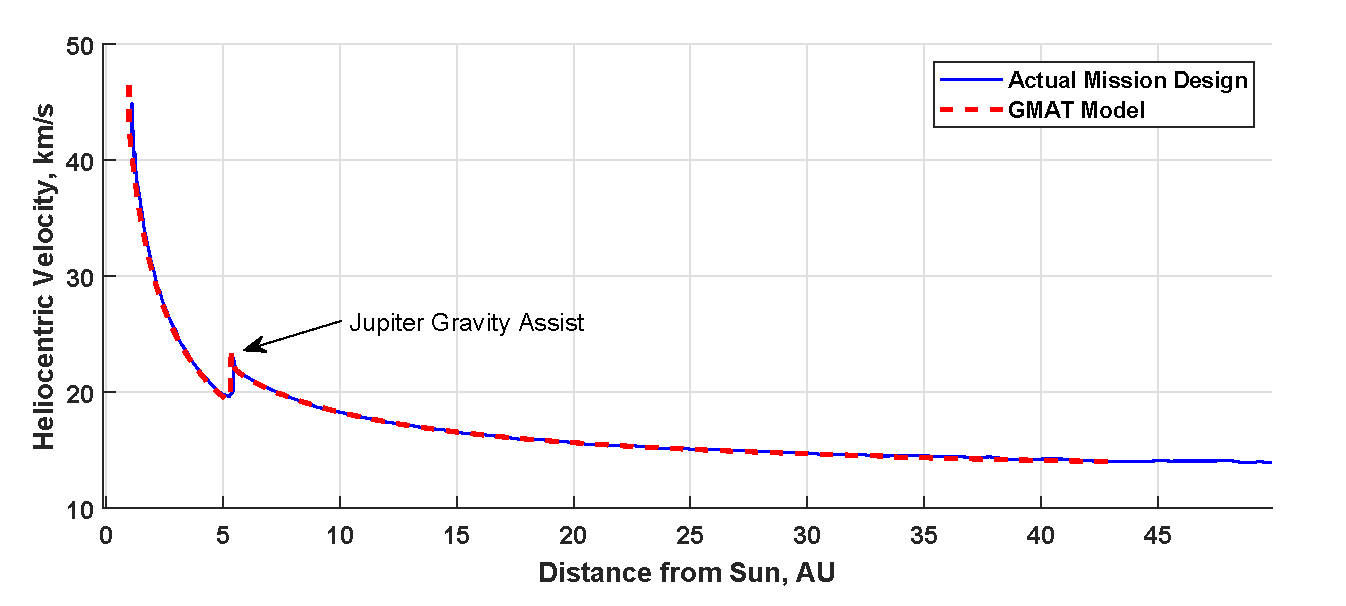
\includegraphics[width=0.85\textwidth]{vel2.eps}
    \caption{Plot comparing New Horizons heliocentric velocity of the actual mission plan and that of the GMAT model \cite{orig}}
    \label{fig:vel}
\end{figure}




%-------------------------------------------------------------------------------
% REFERENCES
%-------------------------------------------------------------------------------
\begin{thebibliography}{}
\bibitem{jhu}"New Horizons : The Path to Pluto and Beyond", Pluto.jhuapl.edu, 2020. [Online]. Available: http://pluto.jhuapl.edu/Mission/The-Path-to-Pluto-and-Beyond.php. [Accessed: 03- Mar- 2020].

\bibitem{soi}R. A. N. Araujo, O. C. Winter, A. F. B. A. Prado, R. Vieira Martins, Sphere of influence and gravitational capture radius: a dynamical approach, Monthly Notices of the Royal Astronomical Society, Volume 391, Issue 2, December 2008, Pages 675–684, https://doi.org/10.1111/j.1365-2966.2008.13833.x

\bibitem{utburn}]"New Horizons Conducts Final Course Correction for New Year’s Day Flyby of Next KBO in 2019", AmericaSpace, 2015. [Online]. Available: https://www.americaspace.com/2015/11/08/new-horizons-conducts-final-course-correction-for-new-years-day-flyby-of-next-kbo-in-2019/. [Accessed: 04- Mar- 2020].

\bibitem{gmat}NASA Goddard Space Flight Center, "General Mission Analysis Tool (GMAT) Mathematical Specifications"; February 2018.
\bibitem{plutoperi}"New Horizons: News Article?page=20150714 2", Pluto.jhuapl.edu, 2015. [Online]. Available: http://pluto.jhuapl.edu/News-Center/News-Article.php?page=20150714-2. [Accessed: 03- Mar- 2020].

\bibitem{jupperi}Y. Guo (Johns Hopkins University Applied Physics Laboratory), B. Williams, F. Pelletier (KinetX), J. McAdams, W.-J. Shyong (APL). "TRAJECTORY MONITORING AND CONTROL OF THE NEW HORIZONS PLUTO FLYBY"; October 2015.

\bibitem{orig}Y. Guo and R. Farquhar, "New Horizons Mission Design", Space Science Reviews, vol. 140, no. 1-4, pp. 49-74, 2007. Available: 10.1007/s11214-007-9242-y.

\end{thebibliography}{}
%-------------------------------------------------------------------------------
% APPENDIX
%-------------------------------------------------------------------------------
\appendix
%\addcontentsline{toc}{section}{APPENDIX}
\renewcommand\thefigure{A.\arabic{figure}}  
\setcounter{figure}{0}



\end{document}




%-------------------------------------------------------------------------------
% SNIPPETS
%-------------------------------------------------------------------------------

% \begin{figure}[!ht]
% 	\centering
% 	\includegraphics[width=0.8\textwidth]{file_name}
% 	\caption{}
% 	\centering
% 	\label{label:file_name}
% \end{figure}

%\begin{figure}[!ht]
%	\centering
%	\includegraphics[width=0.8\textwidth]{graph}
%	\caption{Blood pressure ranges and associated level of hypertension (American Heart Association, 2013).}
%	\centering
%	\label{label:graph}
%\end{figure}

%\begin{wrapfigure}{r}{0.30\textwidth}
%	\vspace{-40pt}
%	\begin{center}
%		\includegraphics[width=0.29\textwidth]{file_name}
%	\end{center}
%	\vspace{-20pt}
%	\caption{}
%	\label{label:file_name}
%\end{wrapfigure}

%\begin{wrapfigure}{r}{0.45\textwidth}
%	\begin{center}
%		\includegraphics[width=0.29\textwidth]{manometer}
%	\end{center}
%	\caption{Aneroid sphygmomanometer with stethoscope (Medicalexpo, 2012).}
%	\label{label:manometer}
%\end{wrapfigure}

%\begin{table}[!ht]\footnotesize
%	\centering
%	\begin{tabular}{cccccc}
%	\toprule
%	\multicolumn{2}{c} {Pearson's correlation test} & \multicolumn{4}{c} {Independent t-test} \\
%	\midrule	
%	\multicolumn{2}{c} {Gender} & \multicolumn{2}{c} {Activity level} & \multicolumn{2}{c} {Gender} \\
%	\midrule
%	Males & Females & 1st level & 6th level & Males & Females \\
%	\midrule
%	\multicolumn{2}{c} {BMI vs. SP} & \multicolumn{2}{c} {Systolic pressure} & \multicolumn{2}{c} {Systolic Pressure} \\
%	\multicolumn{2}{c} {BMI vs. DP} & \multicolumn{2}{c} {Diastolic pressure} & \multicolumn{2}{c} {Diastolic pressure} \\
%	\multicolumn{2}{c} {BMI vs. MAP} & \multicolumn{2}{c} {MAP} & \multicolumn{2}{c} {MAP} \\
%	\multicolumn{2}{c} {W:H ratio vs. SP} & \multicolumn{2}{c} {BMI} & \multicolumn{2}{c} {BMI} \\
%	\multicolumn{2}{c} {W:H ratio vs. DP} & \multicolumn{2}{c} {W:H ratio} & \multicolumn{2}{c} {W:H ratio} \\
%	\multicolumn{2}{c} {W:H ratio vs. MAP} & \multicolumn{2}{c} {\% Body fat} & \multicolumn{2}{c} {\% Body fat} \\
%	\multicolumn{2}{c} {} & \multicolumn{2}{c} {Height} & \multicolumn{2}{c} {Height} \\
%	\multicolumn{2}{c} {} & \multicolumn{2}{c} {Weight} & \multicolumn{2}{c} {Weight} \\
%	\multicolumn{2}{c} {} & \multicolumn{2}{c} {Heart rate} & \multicolumn{2}{c} {Heart rate} \\
%	\bottomrule
%	\end{tabular}
%	\caption{Parameters that were analysed and related statistical test performed for current study. BMI - body mass index; SP - systolic pressure; DP - diastolic pressure; MAP - mean arterial pressure; W:H ratio - waist to hip ratio.}
%	\label{label:tests}
%\end{table}
